\documentclass[9pt,notes]{beamer}
%\documentclass{foils} %if wish to emulate the foils class using beamer

% - Style is ornate.

\mode<presentation>
{
%  \setbeamertemplate{background canvas}[vertical
%shading][bottom=red!10,top=blue!10]

    %% various themes available from the official Beamer user guide
    %\usetheme{default} %% blue, black, and white
    \usetheme{Madrid} %% red, white, and black
    %\usetheme{Frankfurt}
    \usefonttheme[onlysmall]{structurebold}
    %\usefonttheme[onlysmall]{structuresmallcapsserif}

    \setbeamercovered{transparent}
    % or whatever (possibly just delete it)
    %\usecolortheme{beetle}
}

\usepackage{multimedia}
\usepackage[english]{babel}
\usepackage{amsfonts, amsmath, mathrsfs}
\usepackage{amsxtra, amsthm, amssymb, amscd}
\usepackage{float}
\usepackage{graphics}
\usepackage{graphicx}
\usepackage{subcaption}
\usepackage{latexsym}
\usepackage{multimedia}
\usepackage{hyperref}
%\usepackage[dvips]{color} \usepackage{color}
%\usepackage{epsfig}
%\usepackage{mathrsfs}
%\usepackage{rotating}
%\usepackage{wrapfig}
%\usepackage[all]{xy}
%\usepackage{verbatim}

\setbeamercovered{dynamic}

\newcommand{\R}{\mathbb{R}}
\newcommand{\PP}{\mathbb{P}}
\newcommand{\X}{\mathcal{X}}
\newcommand{\Y}{\mathcal{Y}}
\newcommand{\isoa}{\xrightarrow{\sim}}

\DeclareMathOperator*{\argmin}{arg\,min}
\DeclareMathOperator*{\argmax}{arg\,max}
\DeclareMathOperator{\Exp}{Exp}
\DeclareMathOperator{\grad}{grad}
\DeclareMathOperator{\Log}{Log}
\DeclareMathOperator*{\Cor}{Cor}
\DeclareMathOperator*{\diag}{diag}
\DeclareMathOperator*{\rank}{rank}
\DeclareMathOperator{\tr}{trace}

%%%% color-stuff, e.g., \Green{stuff you want to be printed in green}
\definecolor{LightGray}{rgb}{0.94,0.94,0.94}
\definecolor{VeryLightBlue}{rgb}{0.9,0.9,1}
\definecolor{LightBlue}{rgb}{0.8,0.8,1}
\definecolor{DarkBlue}{rgb}{0,0,0.6}
\definecolor{LightGreen}{rgb}{0.88,1,0.88}
\definecolor{MidGreen}{rgb}{0.6,1,0.6}
\definecolor{DarkGreen}{rgb}{0,0.6,0}
\definecolor{VeryLightYellow}{rgb}{1,1,0.9}
\definecolor{LightYellow}{rgb}{1,1,0.6}
\definecolor{MidYellow}{rgb}{1,1,0.5}
\definecolor{VeryLightRed}{rgb}{1,0.9,0.9}
\definecolor{LightRed}{rgb}{1,0.8,0.8}
\definecolor{Red}{rgb}{1,0,0}
\definecolor{Green}{rgb}{0,1,0}
\definecolor{Blue}{rgb}{0,0,1}
\definecolor{Gray}{rgb}{0.5,0.5,0.5}
\definecolor{Black}{rgb}{0,0,0}
\definecolor{White}{rgb}{1,1,1}
\newcommand{\White}[1]{{\color{White}{#1}}}
\newcommand{\VeryLightBlue}[1]{{\color{VeryLightBlue}{#1}}}
\newcommand{\LightBlue}[1]{{\color{LightBlue}{#1}}}
\newcommand{\DarkBlue}[1]{{\color{DarkBlue}{#1}}}
\newcommand{\DarkGreen}[1]{{\color{DarkGreen}{#1}}}
\newcommand{\VeryLightRed}[1]{{\color{VeryLightRed}{#1}}}
\newcommand{\LightRed}[1]{{\color{LightRed}{#1}}}
\newcommand{\Red}[1]{{\color{Red}{#1}}}
\newcommand{\Gray}[1]{{\color{Gray}{#1}}}
\newcommand{\Black}[1]{{\color{Black}{#1}}}
\newcommand{\Blue}[1]{{\color{Blue}{#1}}}
\newcommand{\Green}[1]{{\color{Green}{#1}}}
\newcommand{\LightGray}[1]{{\color{LightGray}{#1}}}


%%% theorem styles %%%%%%%%%
%\theoremstyle{plain}% default \newtheorem{thm}{Theorem}[section]
%\newtheorem{lem}{Lemma}[section]

%\theoremstyle{definition}
%\newtheorem{defn}{Definition}[section] \newtheorem{exmp}{Example}[section]
%\newtheorem{prop}{Proposition}[section] \newtheorem{cor}{Corollary}[section]

%\newtheorem{property}{Property}[section] \newtheorem{algorithm}{Algorithm}[section]

%\restylefloat{figure} \restylefloat{table}

%\usepackage[latin1]{inputenc} or whatever

\usepackage{beramono}

%\usepackage[T1]{fontenc}
% Or whatever. Note that the encoding and the font should match. If T1
% does not look nice, try deleting the line with the fontenc.

\beamertemplatenavigationsymbolsempty

\title[Cake Defense]{Optimized Strict Multiscale Frangi Prefiltering for Segmentation}
\subtitle{Towards an automated PCSVN extraction}

\author[{Luke Wukmer}] % (optional, use only with lots of authors)
{{Luke Wukmer}}%\inst{1}} \and S.~Another\inst{2}}
% - Use the \inst{?} command only if the authors have different
%   affiliation.

\institute[CSULB] % (optional, but mostly needed)
{
  %\inst{1}%
  Advisor: Dr. Jen-Mei Chang\\
  Department of Mathematics and Statistics\\
  California State University, Long Beach\\
  \texttt{lwukmer@gmail.com}
}
\graphicspath{{./figures/abstract_defense/}
              {./figures/abstract_defense/A-raw_targets/}
             }

\date{April 9, 2019}

\titlegraphic{
\includegraphics[height=2cm]{csulb-seal.png}}
\begin{document}

%%% TITLE SLIDE %%%%
\begin{frame} % % % % % % % % % % % % % % % % % % %
  \titlepage
\end{frame}

\section{Introduction}
\begin{frame} % % % % % % % % % % % % % % % % % % % % % % % % %
\AtEndNote{\par}
	\frametitle{Research Goals}
	\begin{columns}[c]
		\begin{column}{0.5\textwidth}
			\begin{figure}
			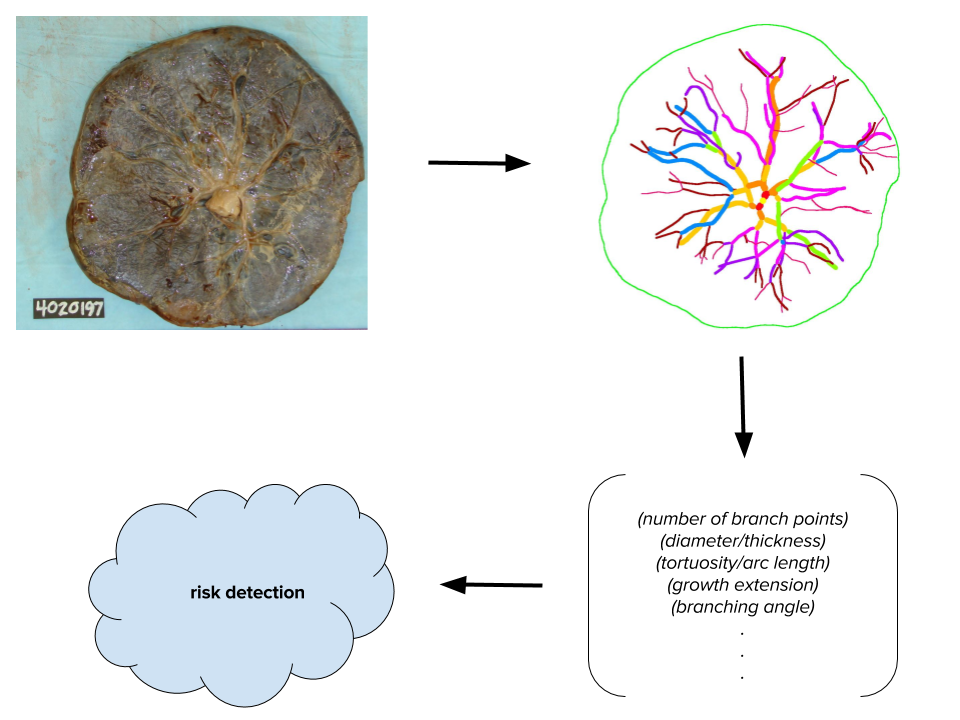
\includegraphics[width=\textwidth]{general_research_question.png}
			\note[item]{In the figure, a manual trace of the placental chorionic
            vascular surface network (PCSVN) is performed.
            This trace is measured in multiple ways. Those measurements are turned into
            a feature vector, which can be used to predict a risk. Refer to Boruta paper.}
			\end{figure}
		\end{column}
		\begin{column}{0.5\textwidth}
			\begin{block}{Vascular Network Extraction in Placentas}
				\begin{itemize}
					\item \textbf{Motivation:}
            Accurate measurement of the vascular structure of a placental sample
            can be used to predict neonatal risk factors, specifically ASD.
					\item \textbf{Challenge:}
						Currently no automated method of obtaining traces of
            PCSVN. Manual tracing is labor intensive but necessary
            for feature analysis.
            \note[item]{Manual tracing requires like 5 hours or something
                  and requires training.
                  There is some guesswork that's done in it too and some limitations
                  in the ground truth itself (will cover later)
                }
					\item \textbf{Research Goal:} Provide a fully automated method of extraction.
          					\end{itemize}
			\end{block}
		\end{column}
	\end{columns}
\end{frame}

\begin{frame}
  \frametitle{The Image Processing Problem}
  \begin{columns}[c]
  \begin{column}{0.5\textwidth}
    \begin{itemize}
        \begin{block}{Our image domain}
        \item The PCSVN is a connected network of veins and arteries
                on the surface of the placenta
        \item We have a ground truth for 201 samples
                from private NCS dataset
        \item Placentas have been formalin-fixed,
                so arteries are more prominent
                (there are issues)
        \item Pictures taken from top down, some glare,
                some inconsistencies.
        \item Placental images are comparatively noisy
        \note[item]{The surface of the placenta has a lot of changes
              in color/topology apart from the PCSVN
              so a lot of techniques that work elsewhere
              for vascular segmentation seem to fail here.
              Thus segmentation is more complicated that than say,
              an eyeball MRI (like original Frangi paper)
            }
      \end{block}
    \begin{block}{Strategy}
      Given the curvilinear nature of these vessels, we will appeal
      to differential geometry.
      \end{block}
    \end{itemize}
  \end{column}
  \begin{column}{0.5\textwidth}
    \centering
    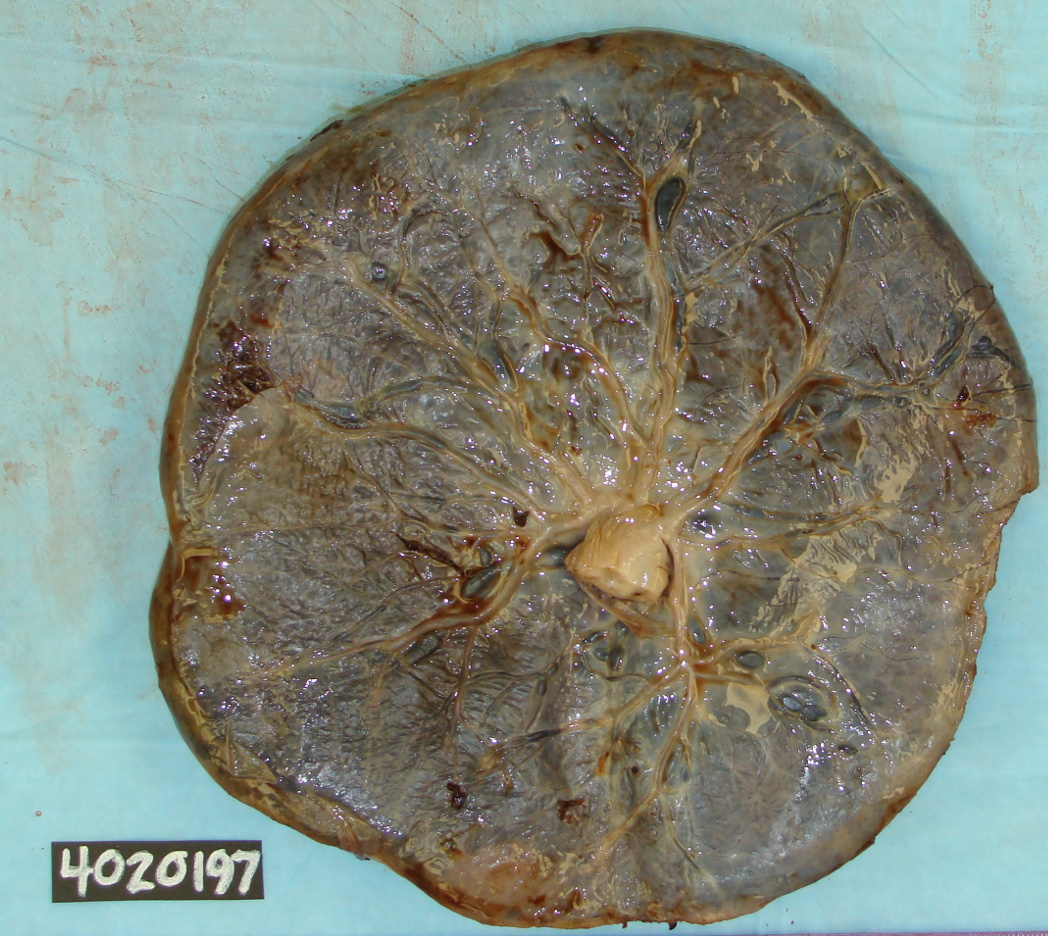
\includegraphics[height=0.36\textheight]{earli_crop.jpg} \\
    {\Huge $\Downarrow$}\\
    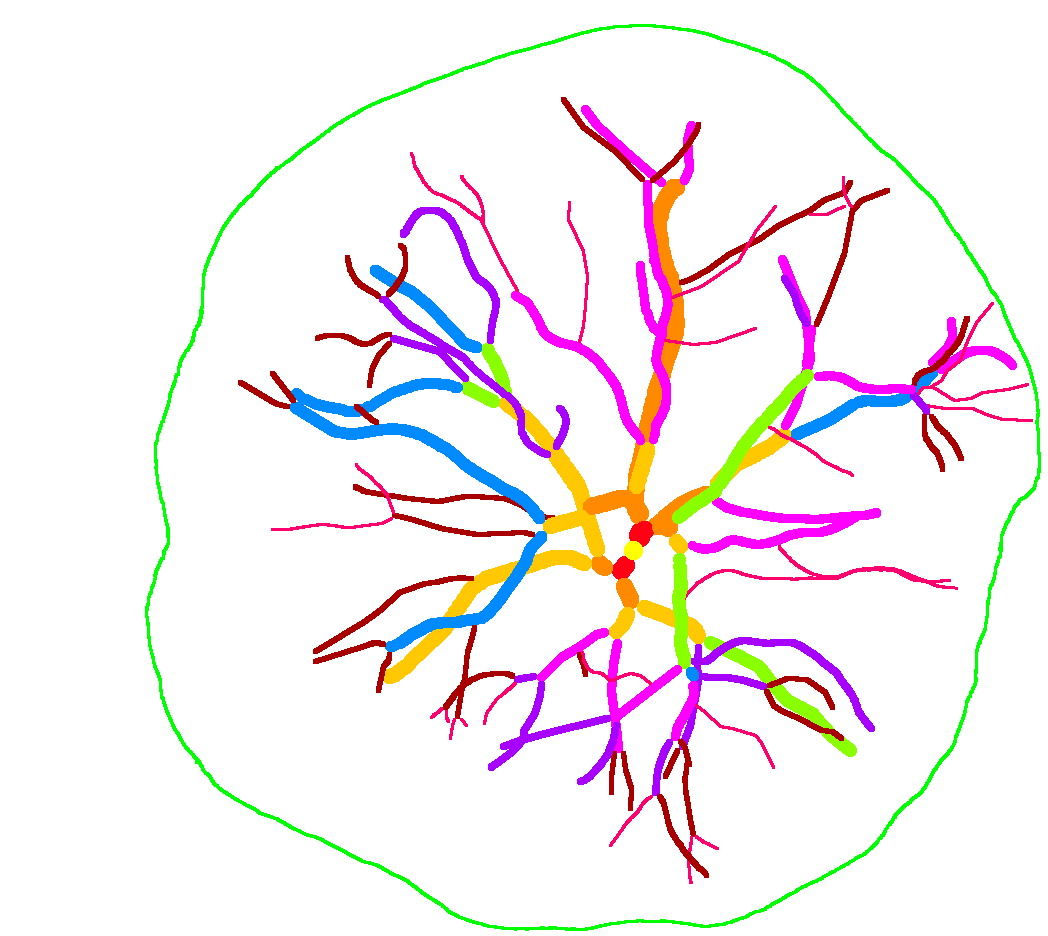
\includegraphics[height=0.36\textheight]{earli_crop_trace.jpg}
    \note[item]{Mention colors are simply vessel widths (3 to 19 odds)
          are part of the tracing protocol. that's really outside of the
          scope of this thesis, but kept anytime we show a ground truth
          because they're pretty
        }
  \end{column}
  \end{columns}
\end{frame}
%SLIDE 2/12 % % % % % % % % % % % % % % % % % % % % % % % % % % % % % % % % % % % % % % % %
%\begin{frame}
%	\frametitle{Previous Research}
%	
%	\begin{enumerate}[\bfseries(a)]
%	\item Nen Huynh used Frangi filtering result (different data set)
%	\item Frangi filtering is followed by morphological filtering (using principal-directions). Agreement with ground truth is displayed. 
%  \item There's a different research group using a cGAN or whatever and it's really good but
%    resource intensive, but whatever maybe just go with that one
%	\end{enumerate}
%	
%	\end{frame}


\section[Math Methods]{Mathematical Methods}
\begin{frame}
\frametitle{Differential Geometry in Image Processing}
  We want to find curvilinear structures in the images, so 
\begin{itemize}
  \item Idealize image as a 3D surface (a graph) with $(x,y)$ spatial coordinates and
        
\end{itemize}
\end{frame}

\begin{frame}
\frametitle{The Frangi Filter}
\end{frame}

\begin{frame}
\frametitle{Implementation Detail: Calculating Discrete Hessian}
\end{frame}
%SLIDE 4/12 % % % % % % % % % % % % % % % % % % % % % % % % % % % % % % % % % % % %
\begin{frame}
\frametitle{Differential Geometry in Image Processing and the Frangi Filter}
\begin{columns}[c]
\begin{column}{0.4\textwidth}
\begin{block}{\footnotesize Principal Curvatures and Principal Directions}
\scriptsize
\begin{gather*}
	\mathsf{L} \in \R^{m\times n} \; \Longleftrightarrow L \in \mathcal{C}^2\Big([0,m] \times [0,n]\Big)\\
	\mathsf{H}(x,y) = \begin{bmatrix} L_{xx} & L_{xy} \\ L_{yx} & L_{yy} \end{bmatrix} \\
	\kappa_i , u_i \; \,\text{for}\; i=1,2
	\intertext{such that}
	\mathsf{H} u_i = \kappa_i u_i \;,\;
	\left|\kappa_1\right| < \left|\kappa_2\right|
\end{gather*}
\end{block}

\begin{block}{\footnotesize Frangi Filter Measure}
	\tiny
	\begin{equation}
	F \{\cdot\} =
	\begin{cases}
	0 & \text{if} \kappa_2 < 0, \\
	\exp \left(\frac{-A^2}{2\beta^2}\right)
		\left(1 - \exp\left( \frac{-S^2}{2c^2}\right)\right) & \textrm{else} \end{cases}
	\end{equation}
	
	\begin{equation}
	S = \sqrt{\kappa_1^2 + \kappa_2^2} \quad\text{(structureness)}
	\end{equation}	
	\begin{equation}
	A = \left|\frac{{\kappa_1}}{\kappa_2}\right| \quad\text{(anisotropy)}
	\end{equation}
	\qquad \qquad with $\beta$, c, parameters
	\end{block}
\end{column}
\begin{column}{0.55\textwidth}
\begin{figure}[h]
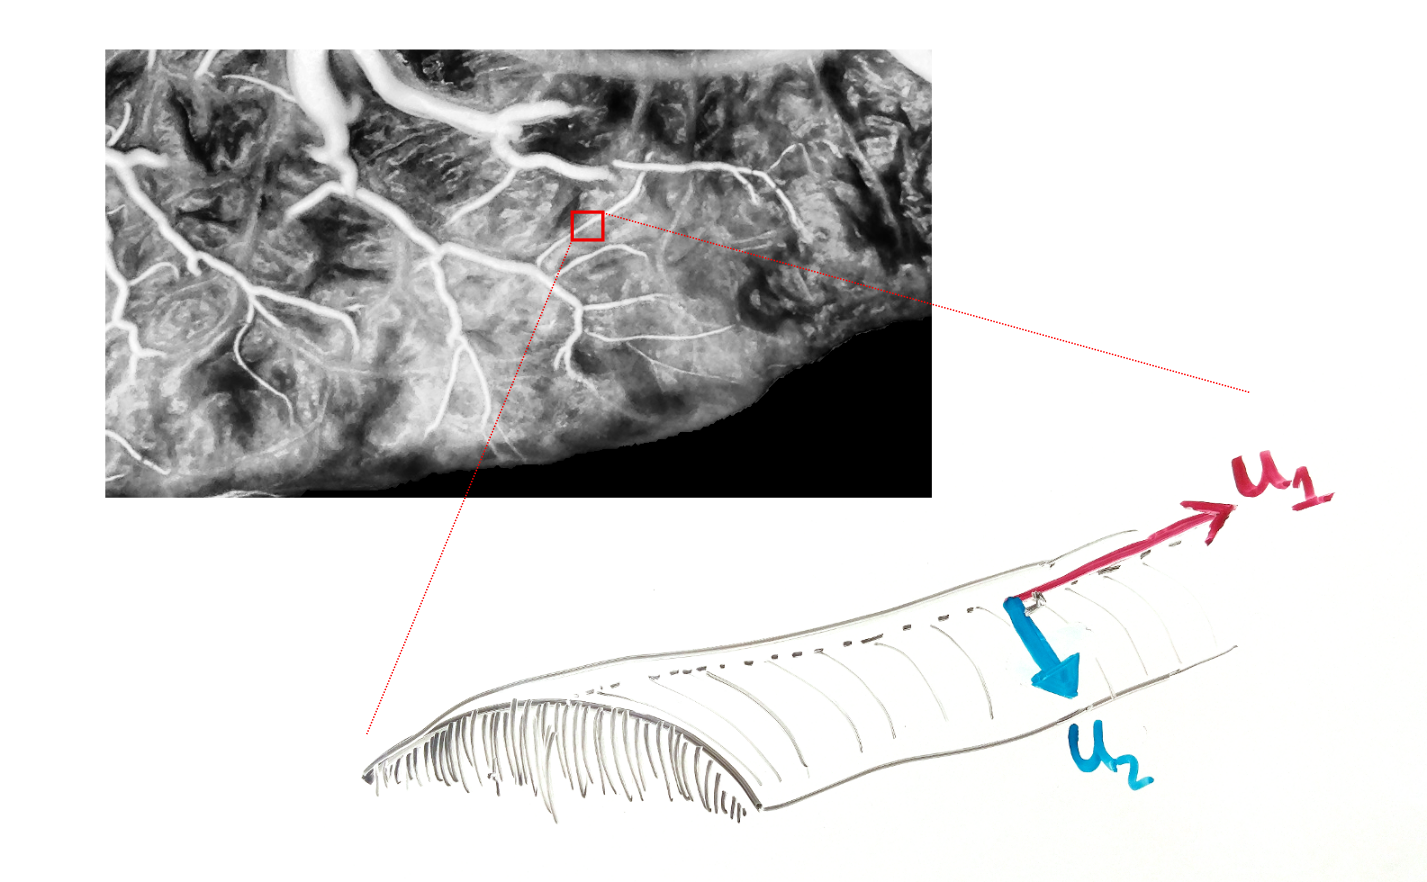
\includegraphics[width=\textwidth]{svginset}
\caption{\footnotesize{The principal curvatures (eigenvectors of the Hessian matrix) point in the direction of greatest and least curvature at each pixel}}
\end{figure}

The Frangi filter \Blue{[2]} finds tubular structures on the surface. Corresponds to areas where $\kappa_2$ is large and $\kappa_1$ is small.

\end{column}
\end{columns}
\end{frame}
%SLIDE 2/12 % % % % % % % % % % % % % % % % % % % % % % % % % % % % % % % % % % % % % % % %
\begin{frame}
	\frametitle{Improved Parameters for Frangi Filter}
	\begin{figure}
		\begin{subfigure}[t]{0.33\textwidth}
			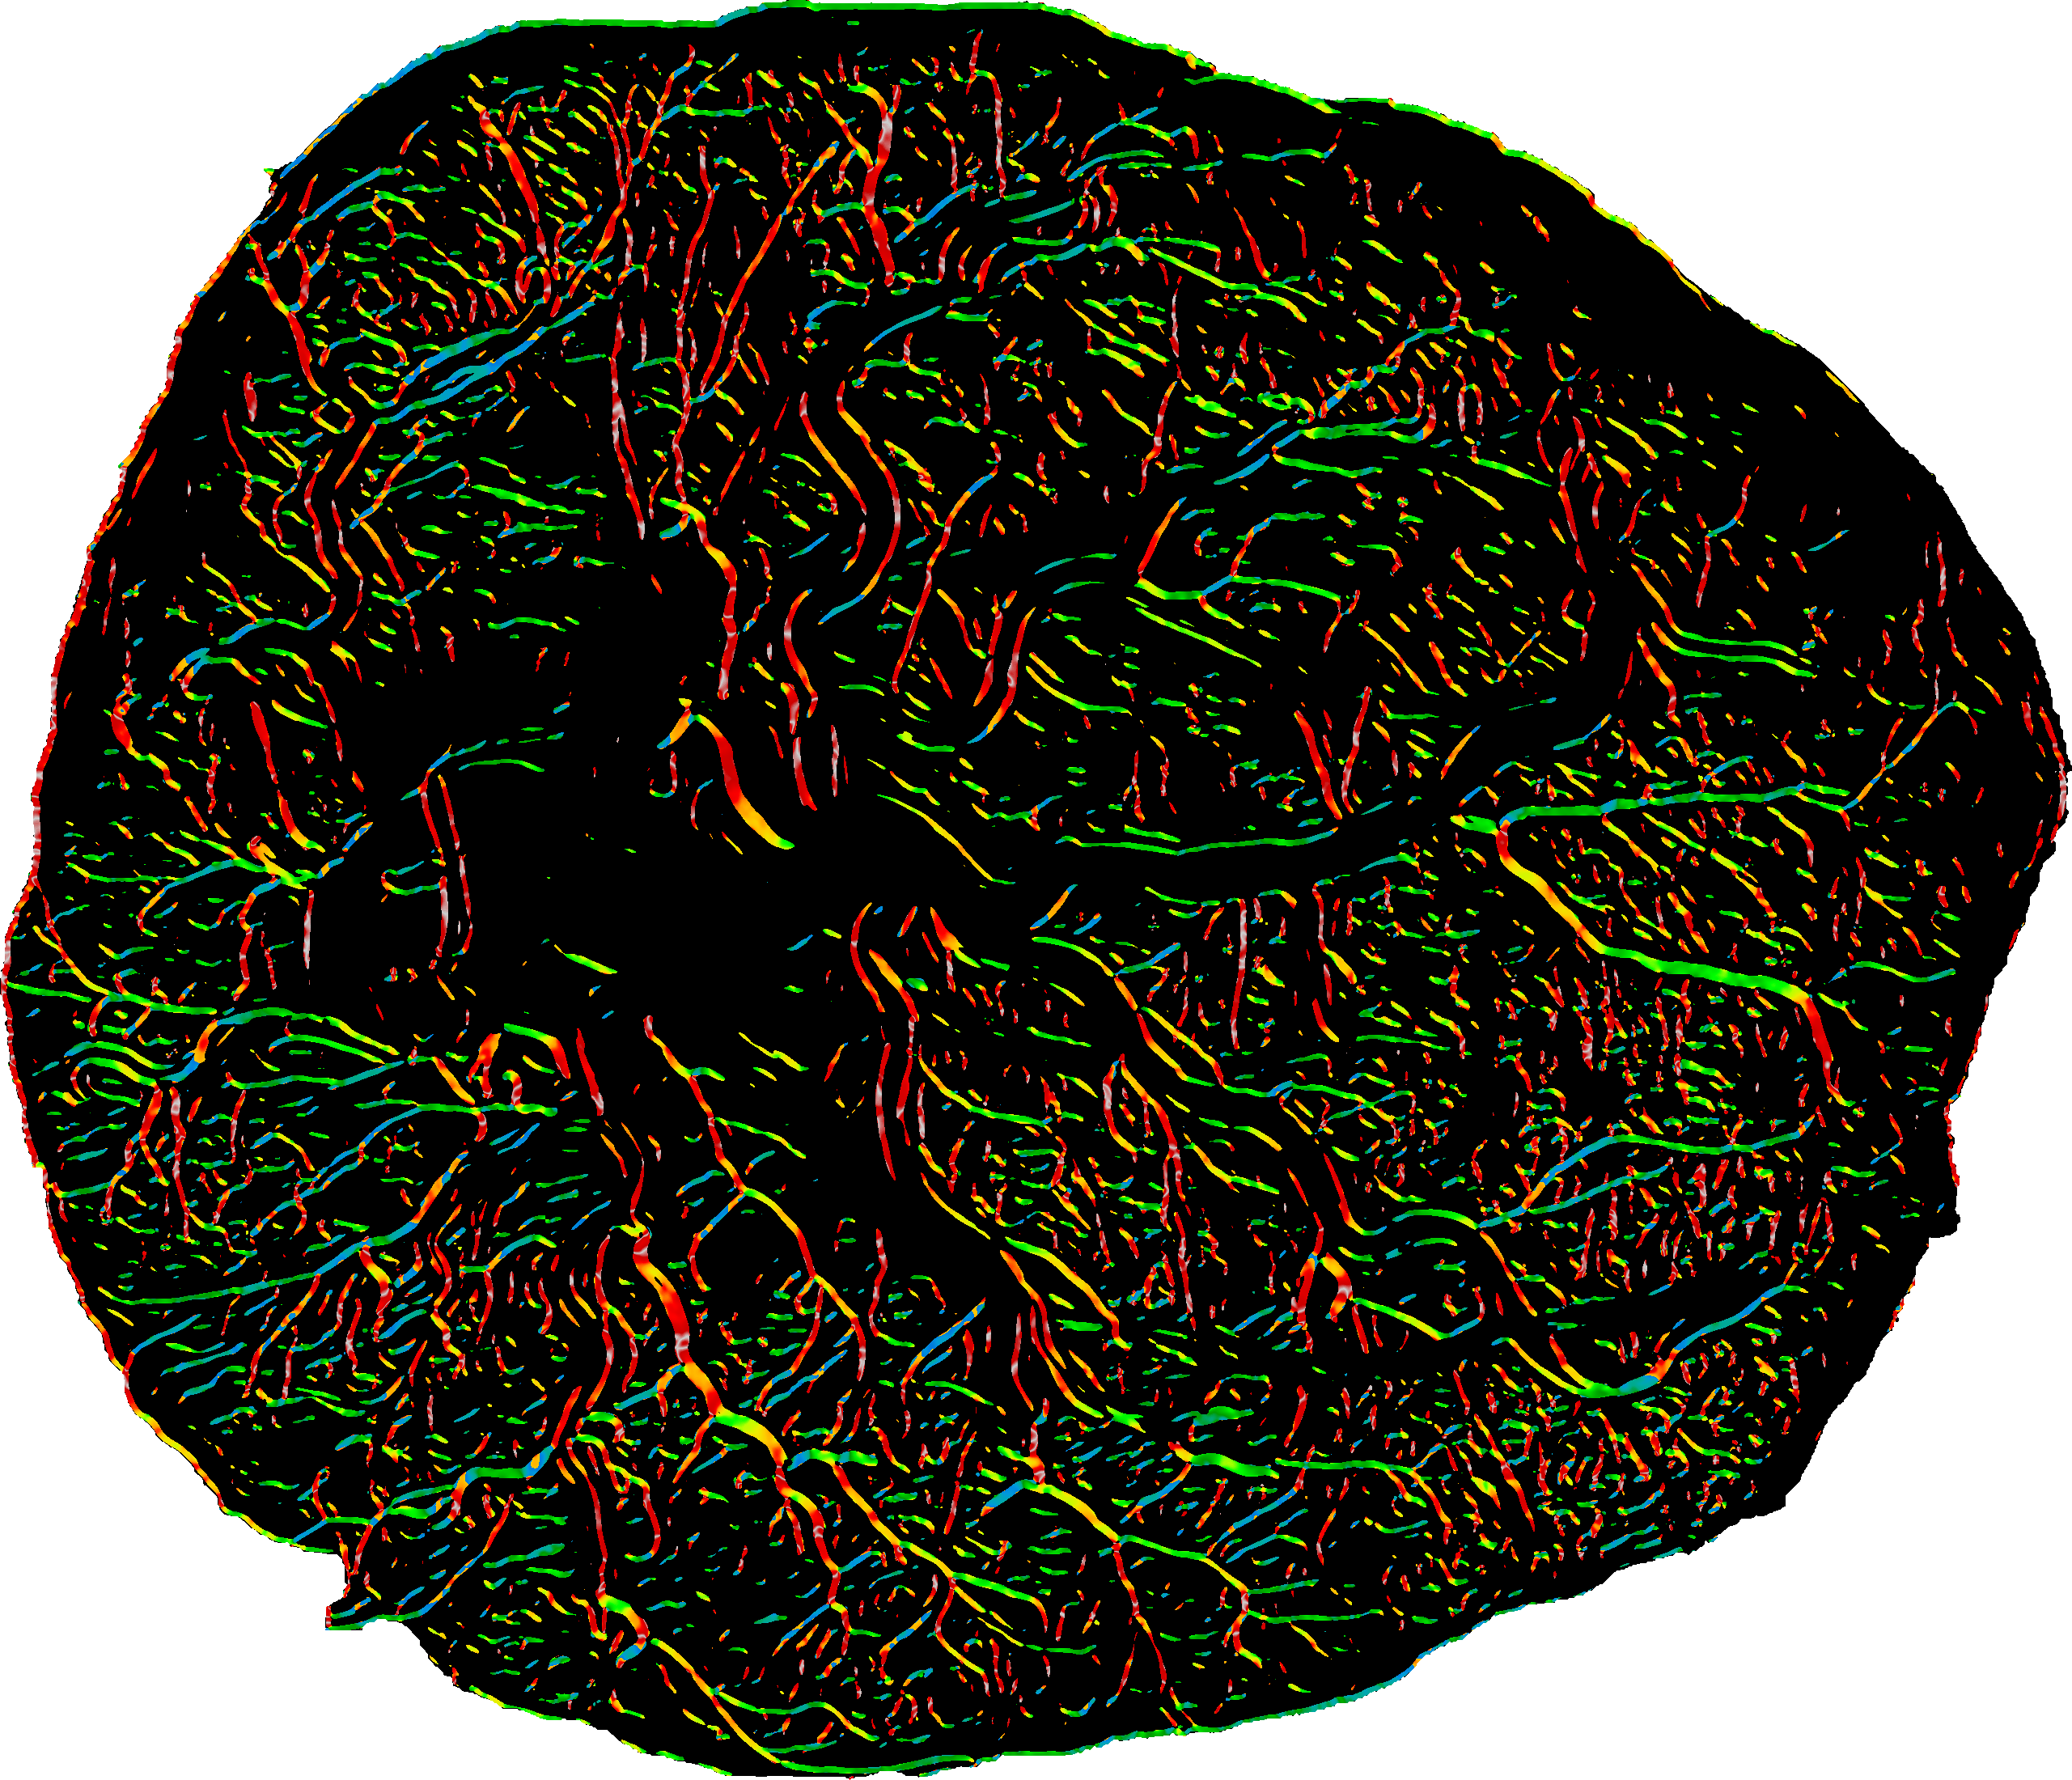
\includegraphics[width=\textwidth]{04-raw.png}
			\caption{Placental sample (bad parameters)}
		\end{subfigure}
		\begin{subfigure}[t]{0.33\textwidth}
			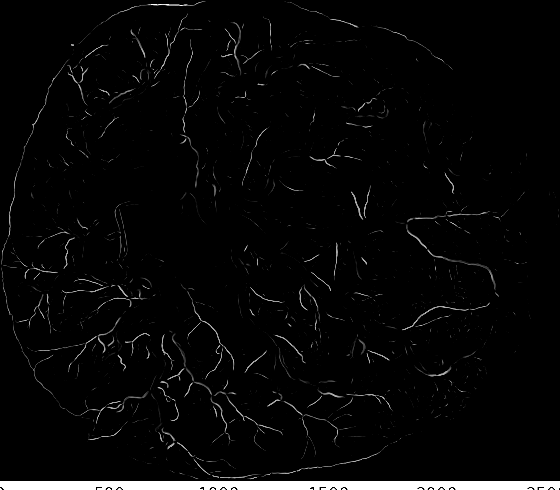
\includegraphics[width=\textwidth]{04-improved.png}
			\caption{improved parameters}
		\end{subfigure}
		\begin{subfigure}[t]{0.33\textwidth}
			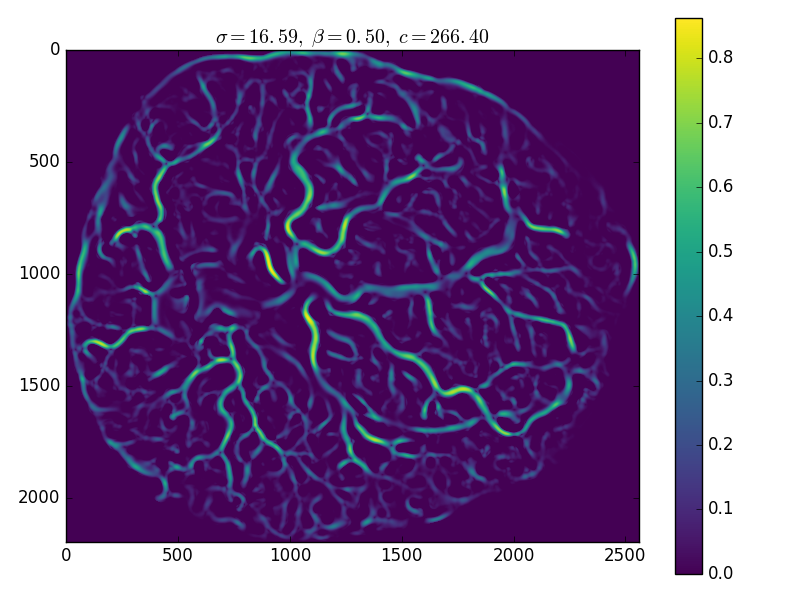
\includegraphics[width=\textwidth]{16.png}
			\caption{improved parameters (larger scale space)}
		\end{subfigure}
	\end{figure}

\end{frame}


\begin{frame} 
	\frametitle{Future Work}
\begin{columns}[c]
\begin{column}{0.5\textwidth}
\begin{figure}
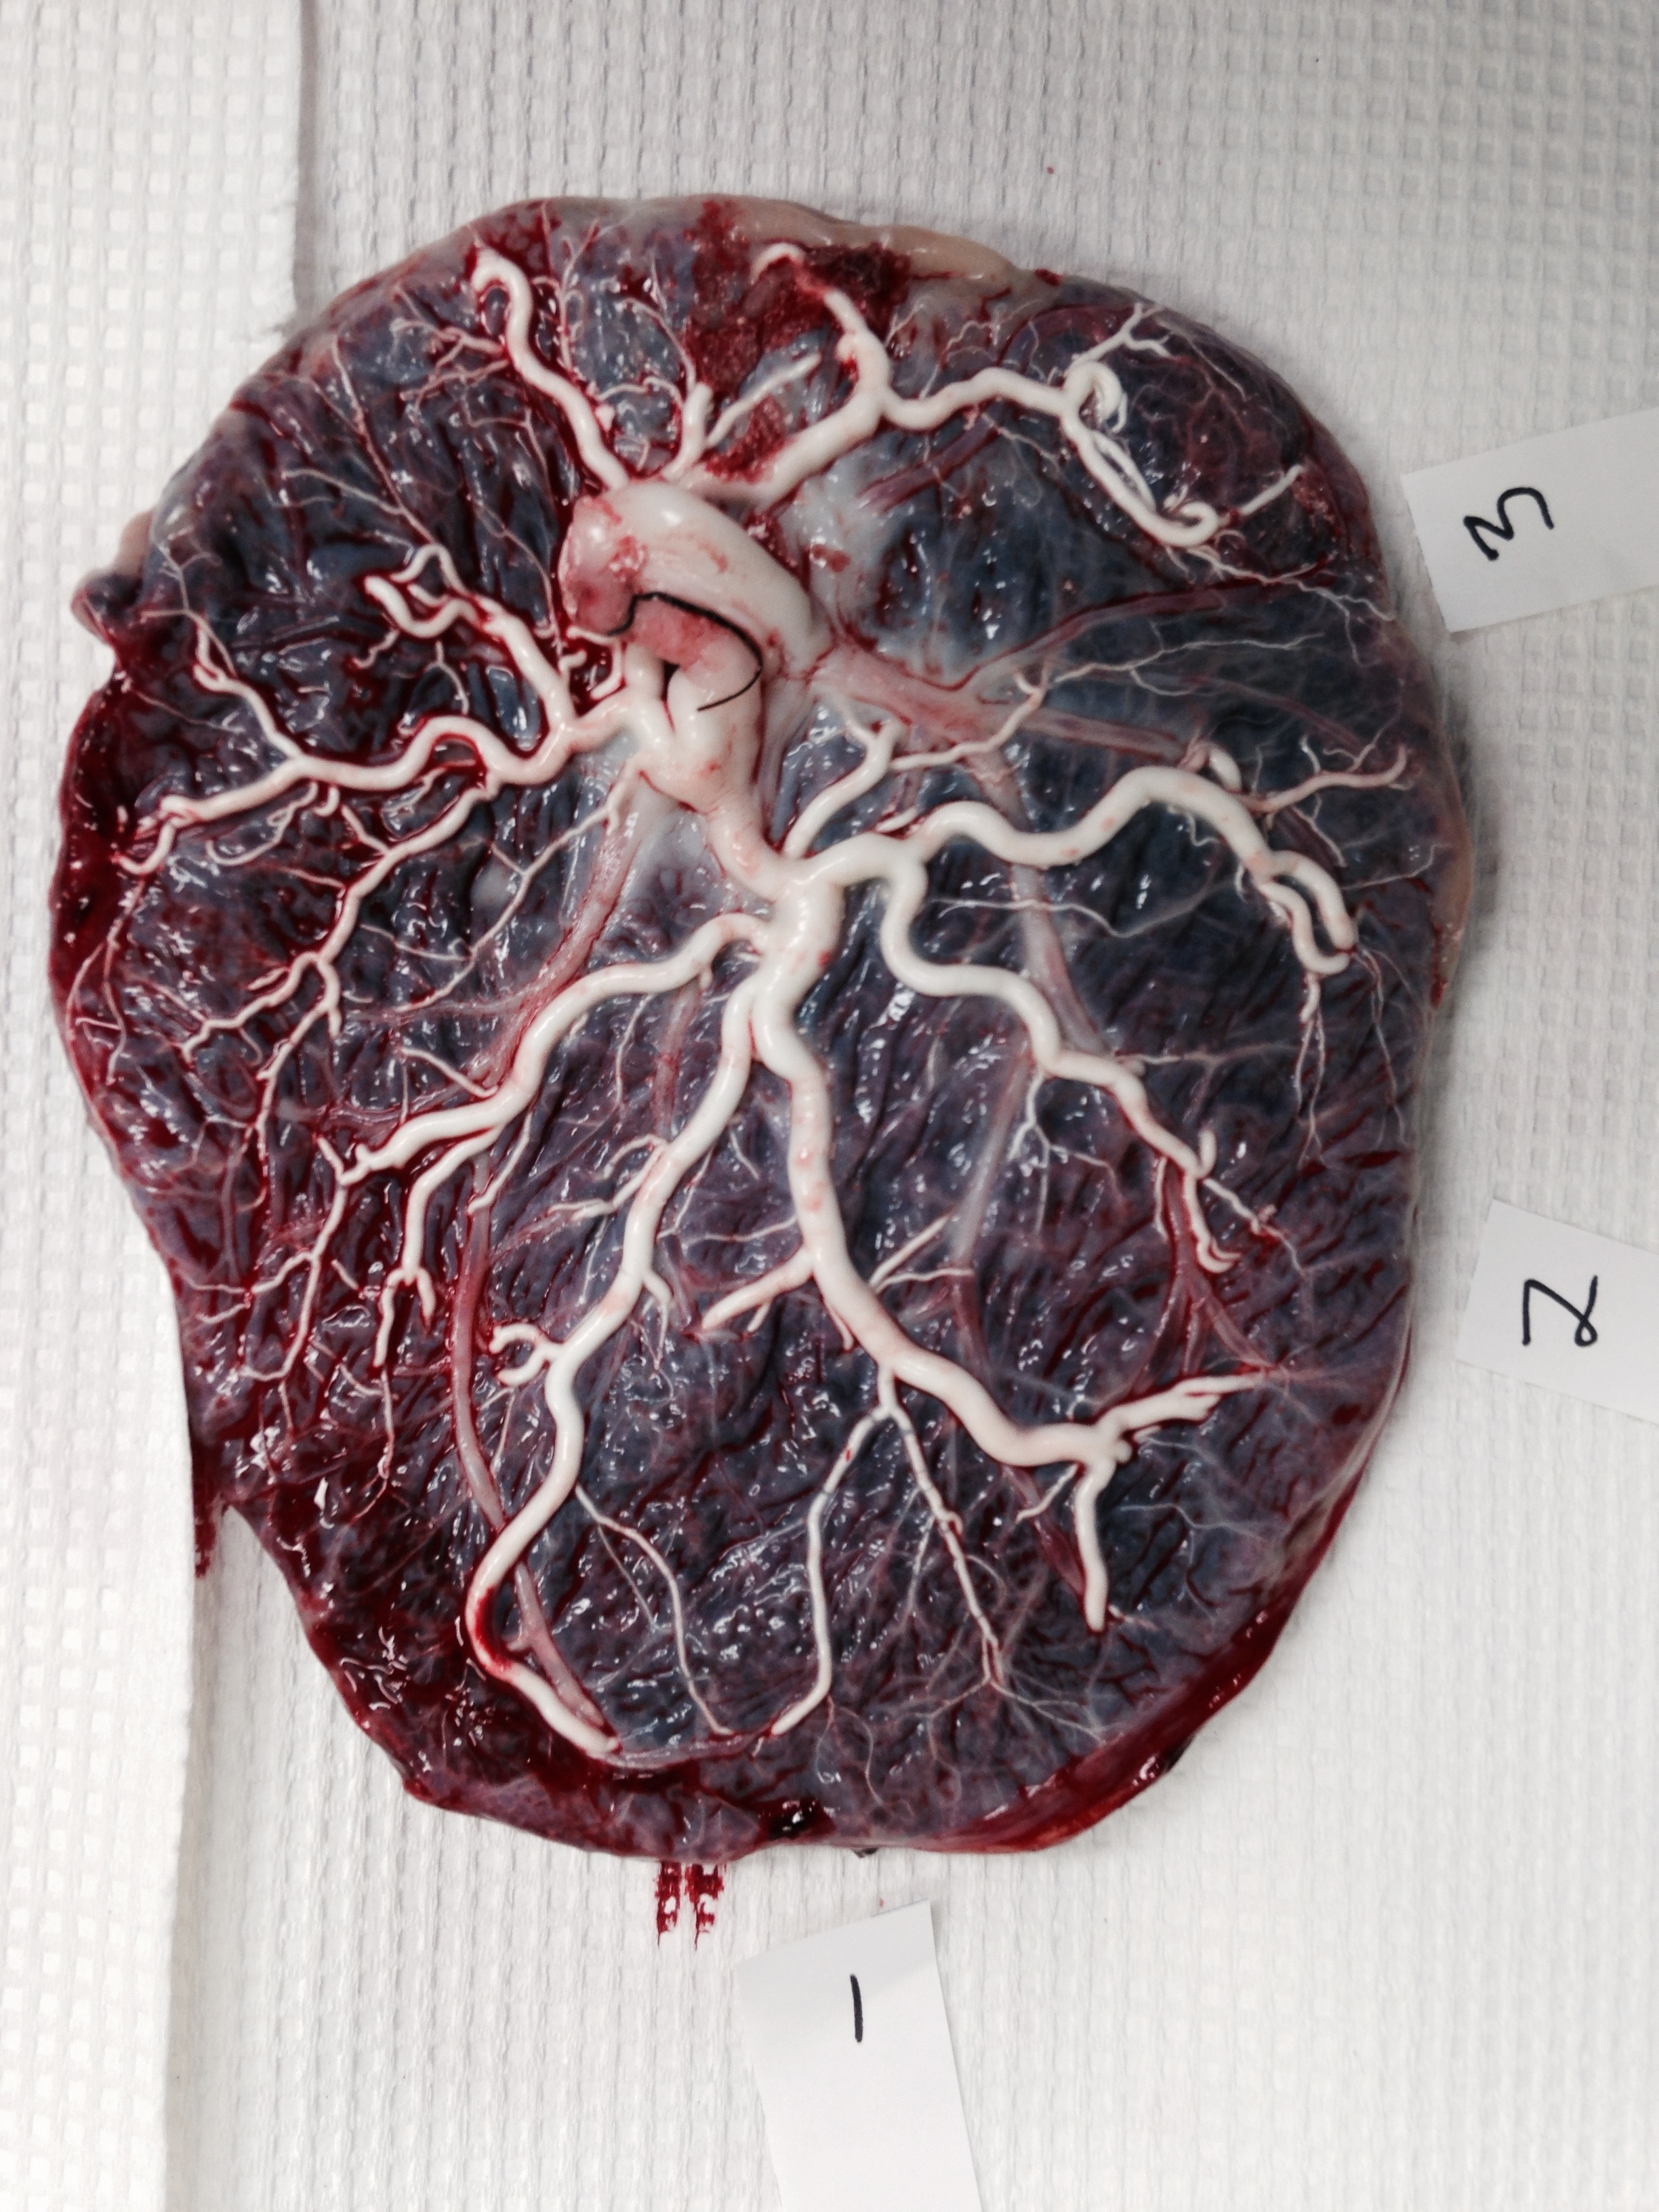
\includegraphics[height=0.45\textheight]{nb}
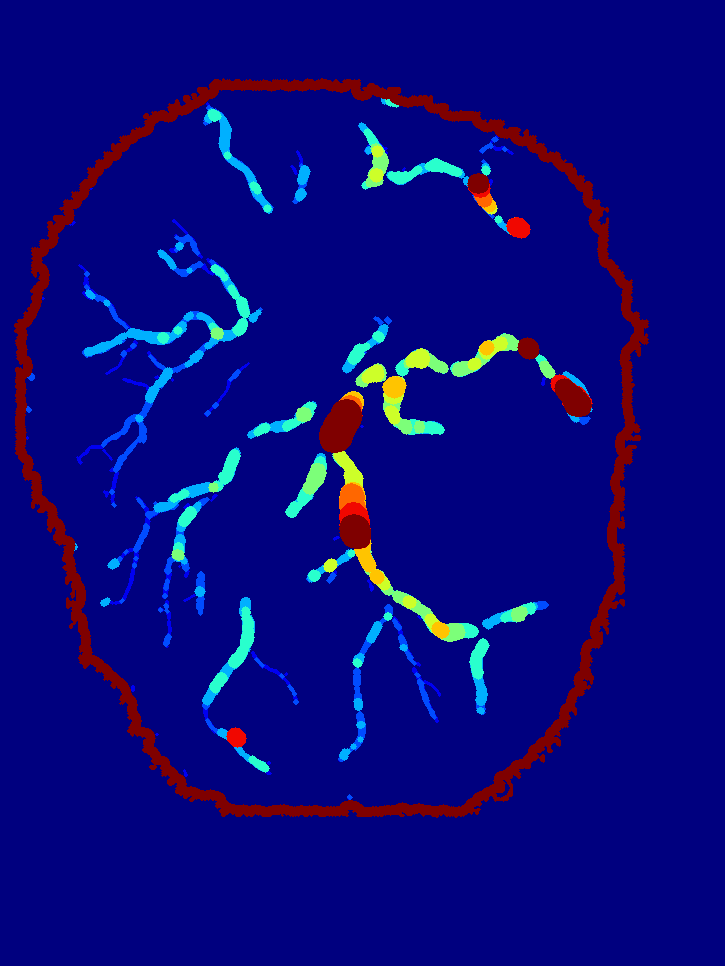
\includegraphics[height=0.45\textheight]{nb_on_skel_labeled}
\end{figure}
\end{column}
\begin{column}{0.4\textwidth}
\textbf{Additional Work Required}
\begin{itemize}
\item Extend to other samples and image domains.
\begin{itemize}
	\item new barium samples
	\item other placental samples (NCS, EARLI)
	\item STARE, DRIVE retinal database
	\item other curvilinear image sets?
	
\end{itemize}
\item Adapt previous morphological filtering to improved frangi targets
\item Speedups with FFT (completed!)
\item Find good way to quantify results
\item Graph connection problem, etc.

\end{itemize}

\end{column}
\end{columns}
\end{frame}

\begin{frame}
	\frametitle{Appendix: Main Extraction Process}
	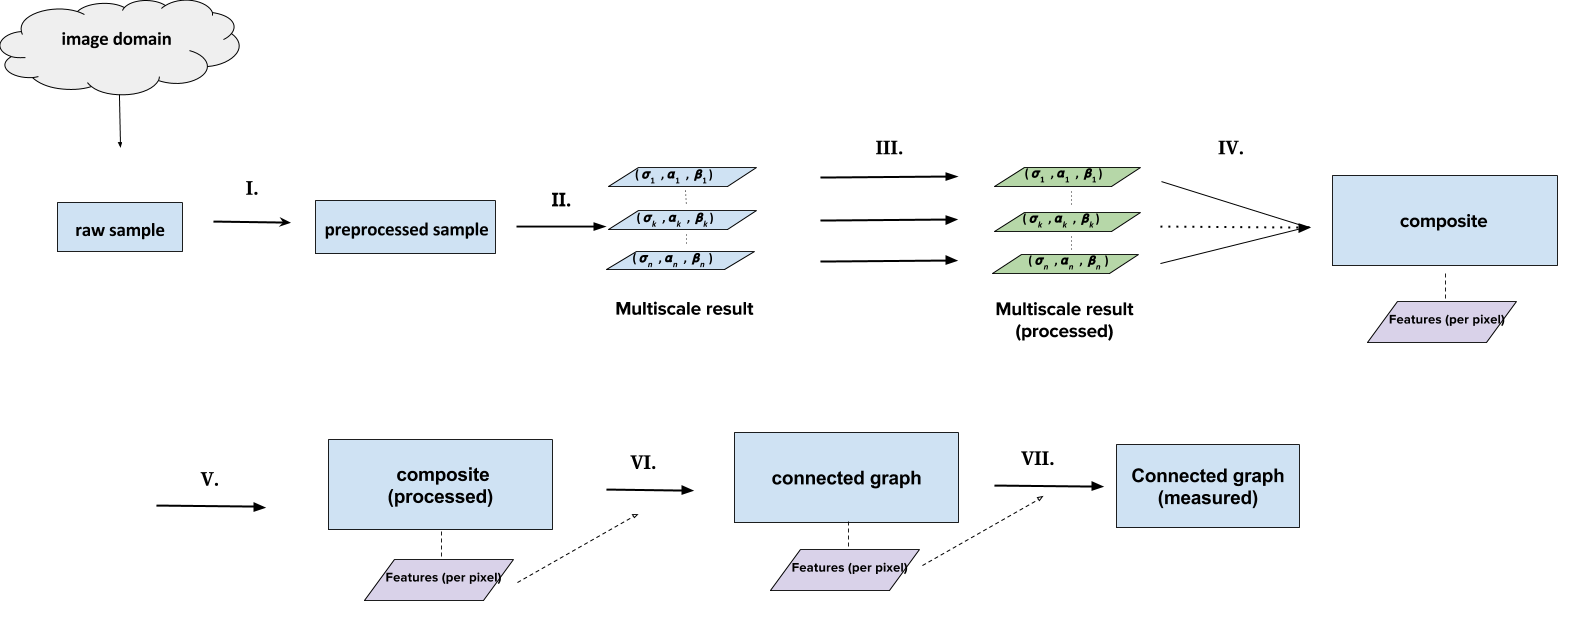
\includegraphics[width=\textwidth]{main_flowchart}
\end{frame}
%SLIDE 8 % % % % % % % % % % % % % % % % % % % % % % % % % % % % % % % % % % % % %
\begin{frame}
	\frametitle{Principal Directions with Frangi Filter (Example with  $\sigma=2$)}
	\begin{figure}
		\centering
		\begin{subfigure}[b]{0.30\textwidth}
			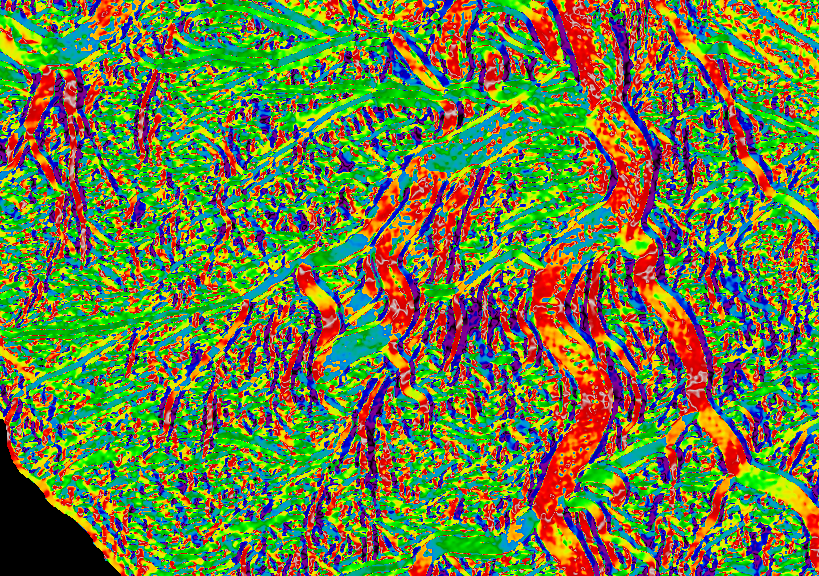
\includegraphics[width=\textwidth]{02pdall-inset}
			\caption{all $\theta(u_2 , e_1)$}
		\end{subfigure}
		\begin{subfigure}[b]{0.30\textwidth}
			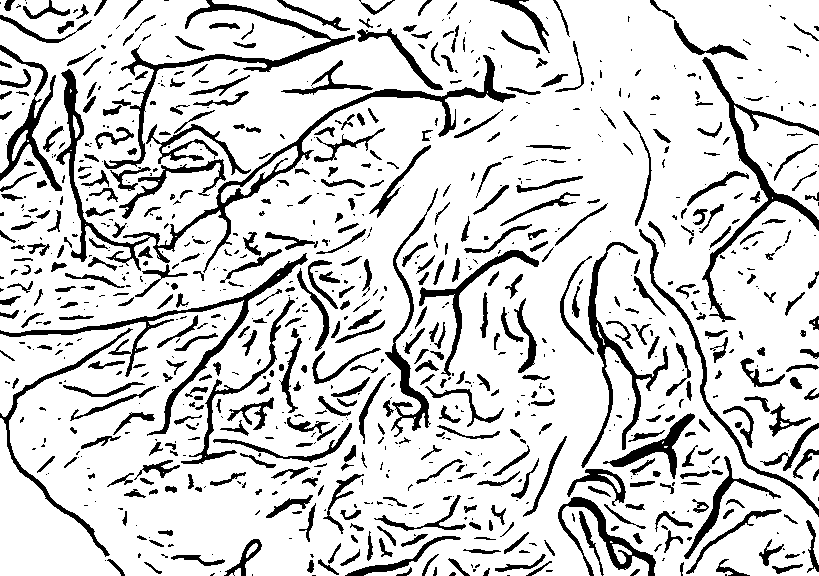
\includegraphics[width=\textwidth]{02bw-inset}
			\caption{Frangi targets}
		\end{subfigure}
		\begin{subfigure}[b]{0.30\textwidth}
			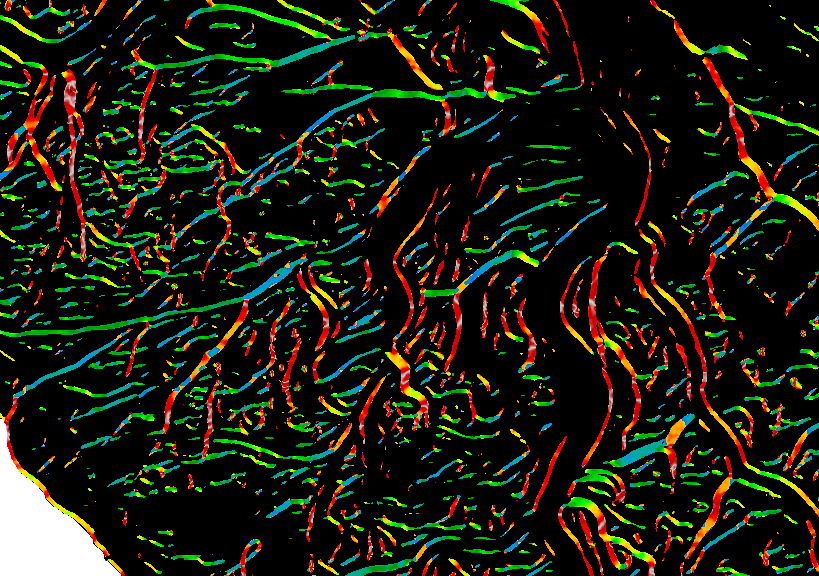
\includegraphics[width=\textwidth]{02pd-inset}
			\caption{frangi targets with $\theta$}
		\end{subfigure}
	\end{figure}
	\begin{columns}[c]
		\begin{column}{0.5\textwidth}
			\begin{figure}
				
\includegraphics[height=0.4\textheight]{morphfilter}
			\end{figure}
		\end{column}
		\begin{column}{0.5\textwidth}
			
			\begin{block}{Morphological Filter}
				\begin{itemize}
					\item Rectangular filter rotated by $\theta(u_1,e_1)$
					\item Rectangle size dependent on $\sigma$ (scale size)
					\item Binary closing $\rightarrow$ binary opening with disk
				\end{itemize}
			\end{block}
		\end{column}
	\end{columns}
\end{frame}

%SLIDE 9/12 % % % % % % % % % % % % % % % % % % % % % % % % % % % % % % % % % % % % % % %
\begin{frame}
	\frametitle{Skeletonization \& Sieving}
	\begin{block}{Morphological Filtering Algorithm}
		\begin{enumerate}[\bfseries(a)]
			\item Join all scales.
			\item Skeletonize.
			\item Iterate over each scale extraction and keep content only if it is connected to the skeleton.
		\end{enumerate}
	\end{block}
	\begin{figure}
		\begin{subfigure}[b]{0.30\textwidth}
			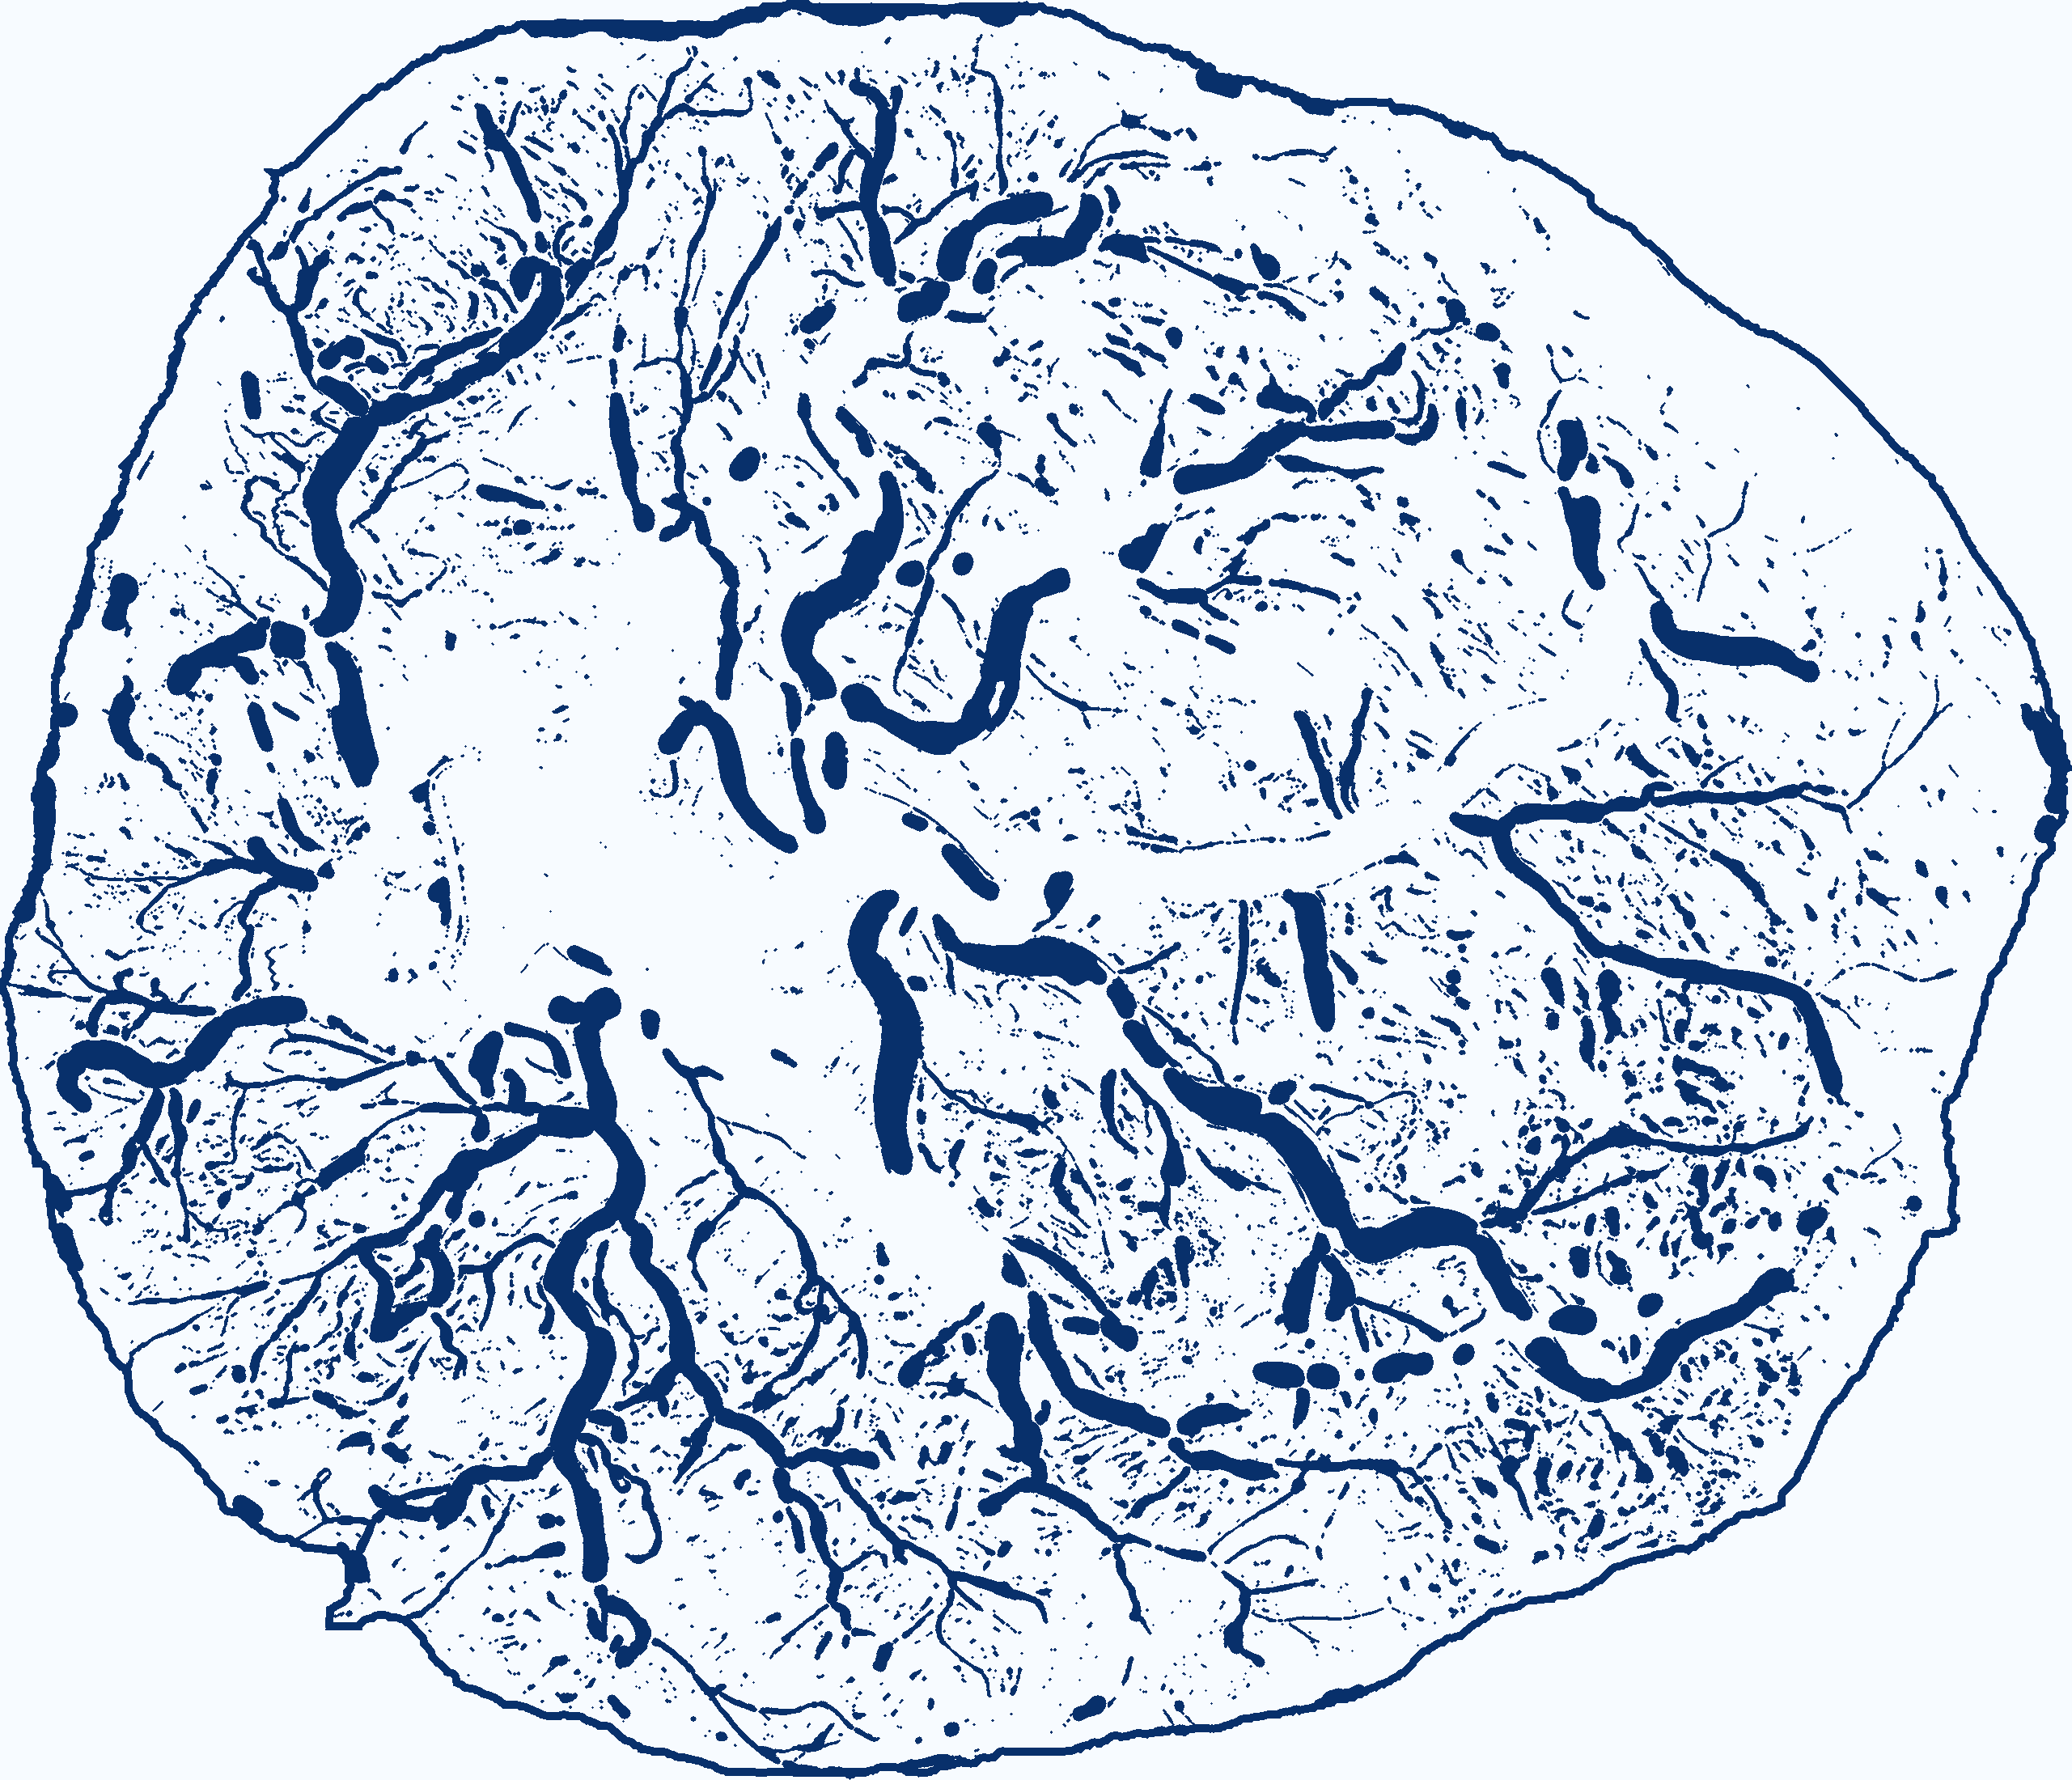
\includegraphics[width=\textwidth]{D-cumulative_binary}
			\caption{Union of all scales}
		\end{subfigure}
		\begin{subfigure}[b]{0.30\textwidth}
			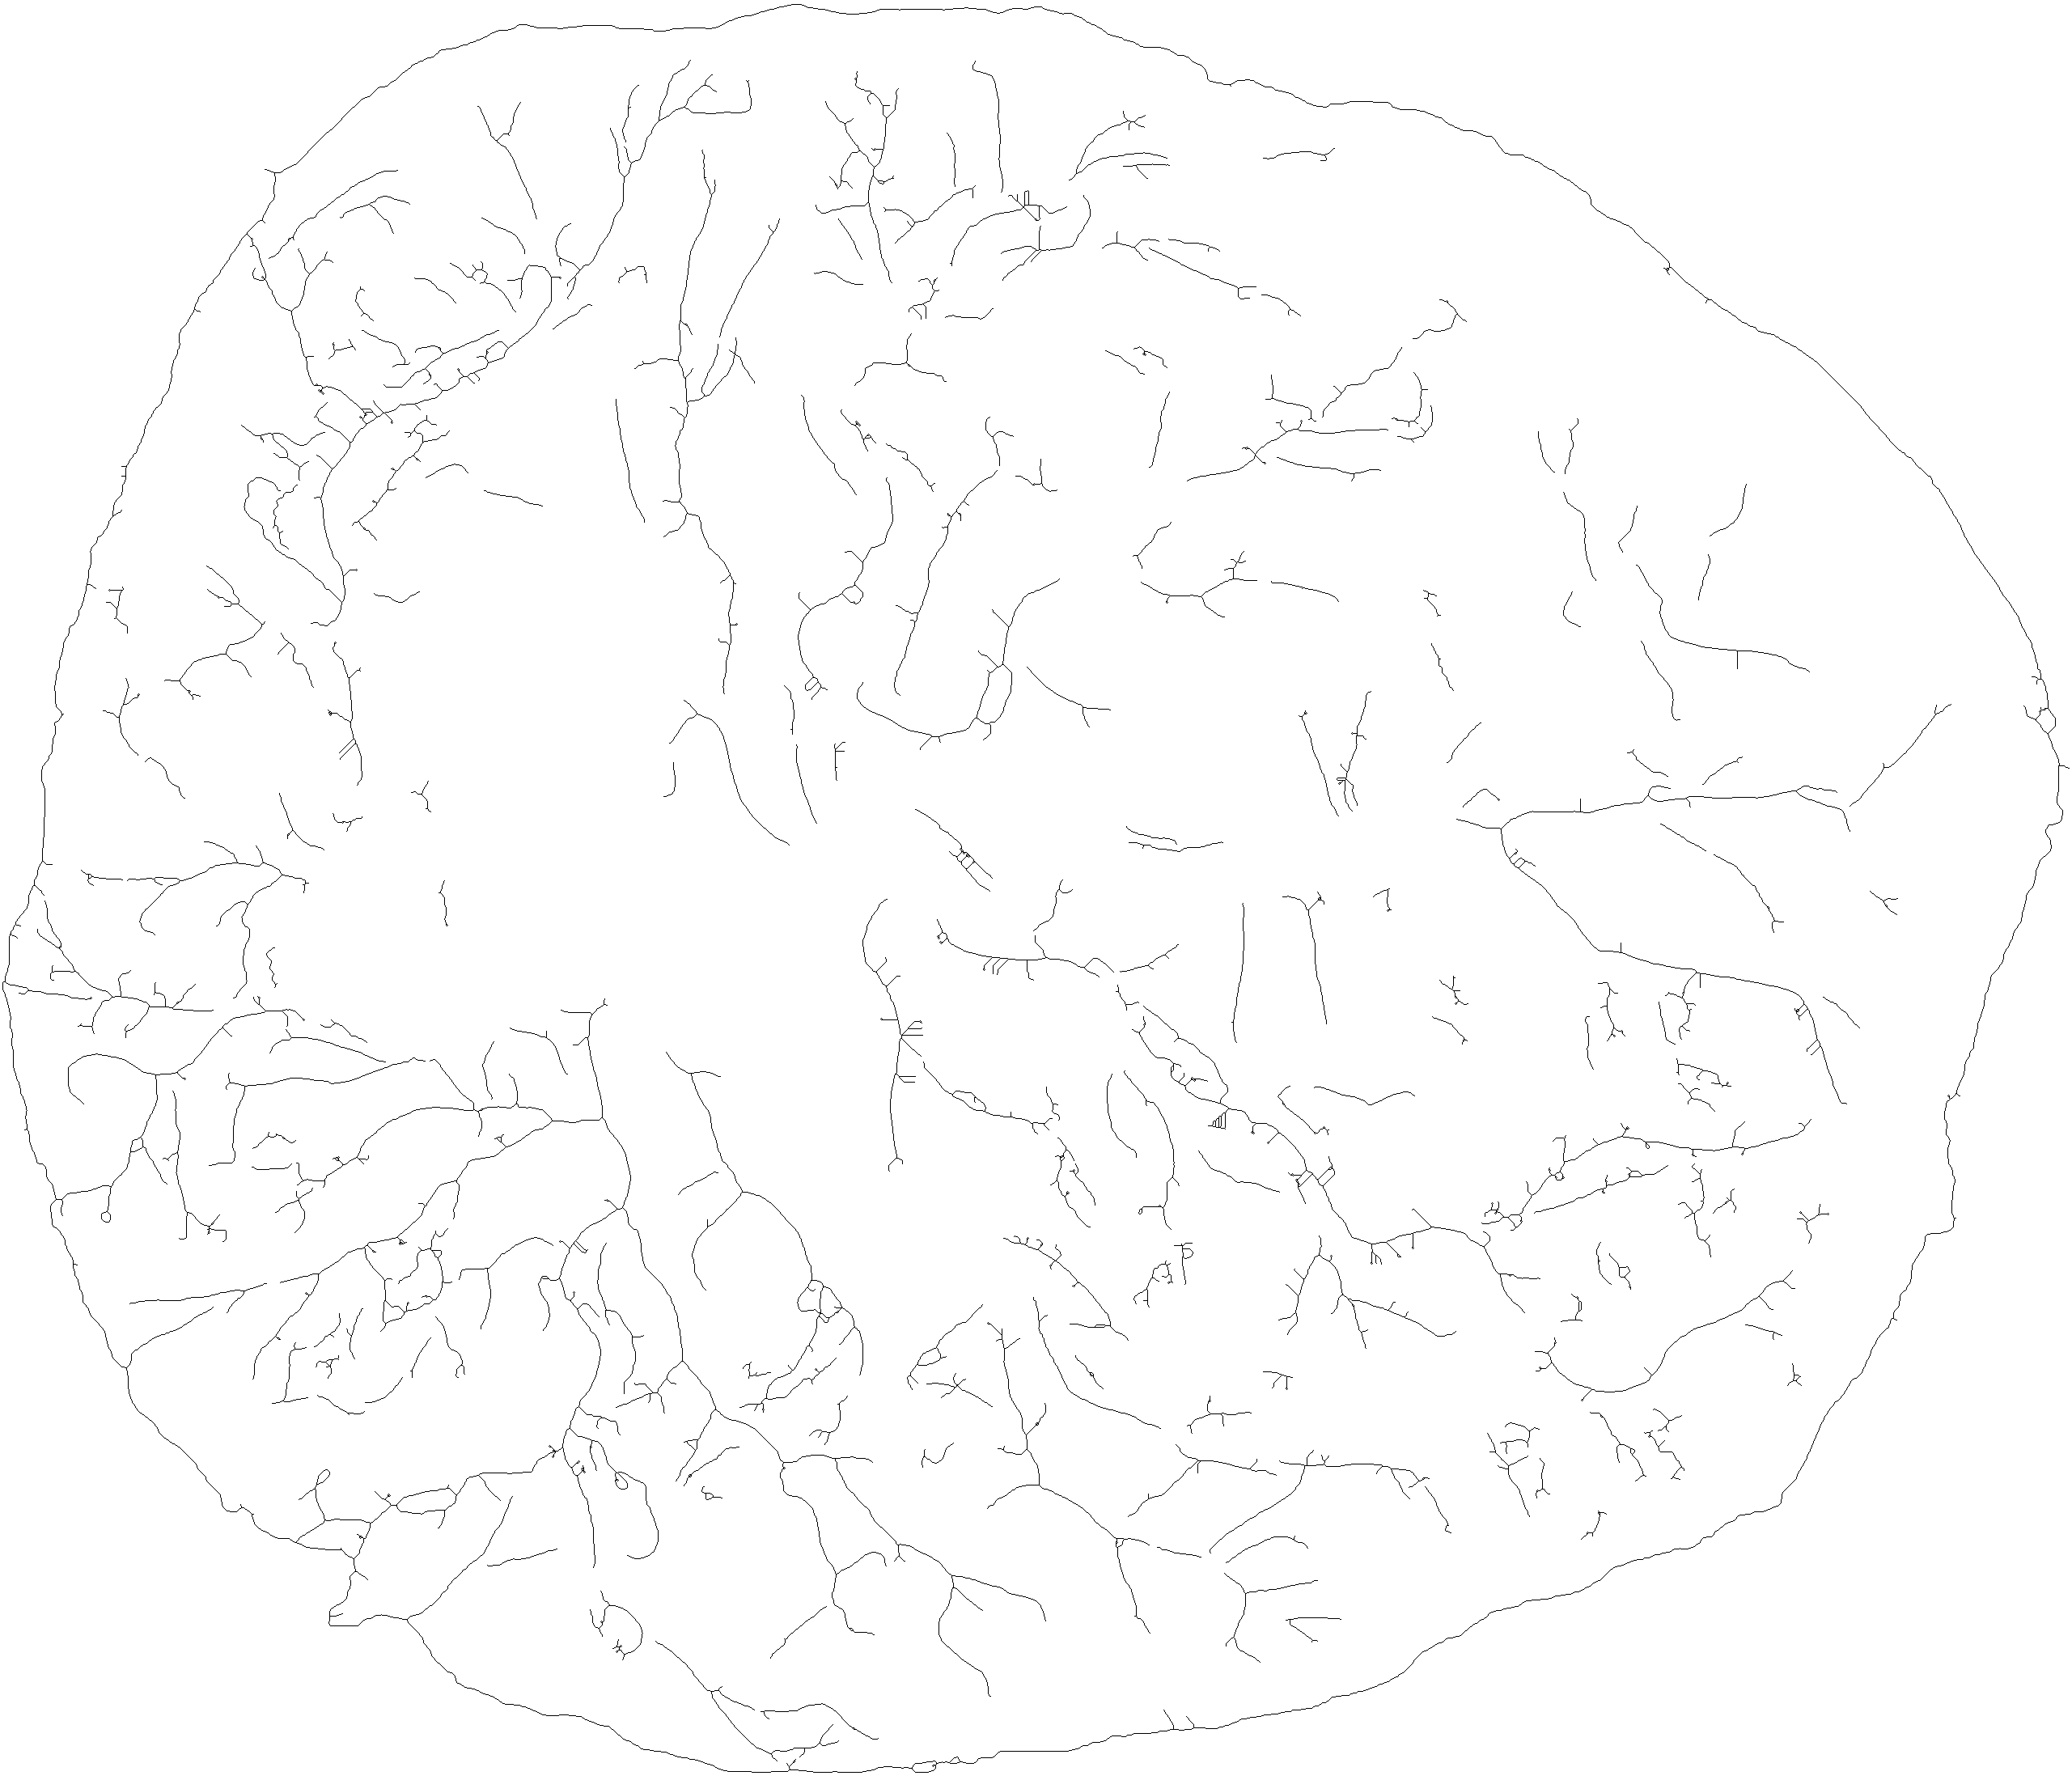
\includegraphics[width=\textwidth]{F-small_skel}
			\caption{Skeletonization of (a)}
		\end{subfigure}
		\begin{subfigure}[b]{0.30\textwidth}
			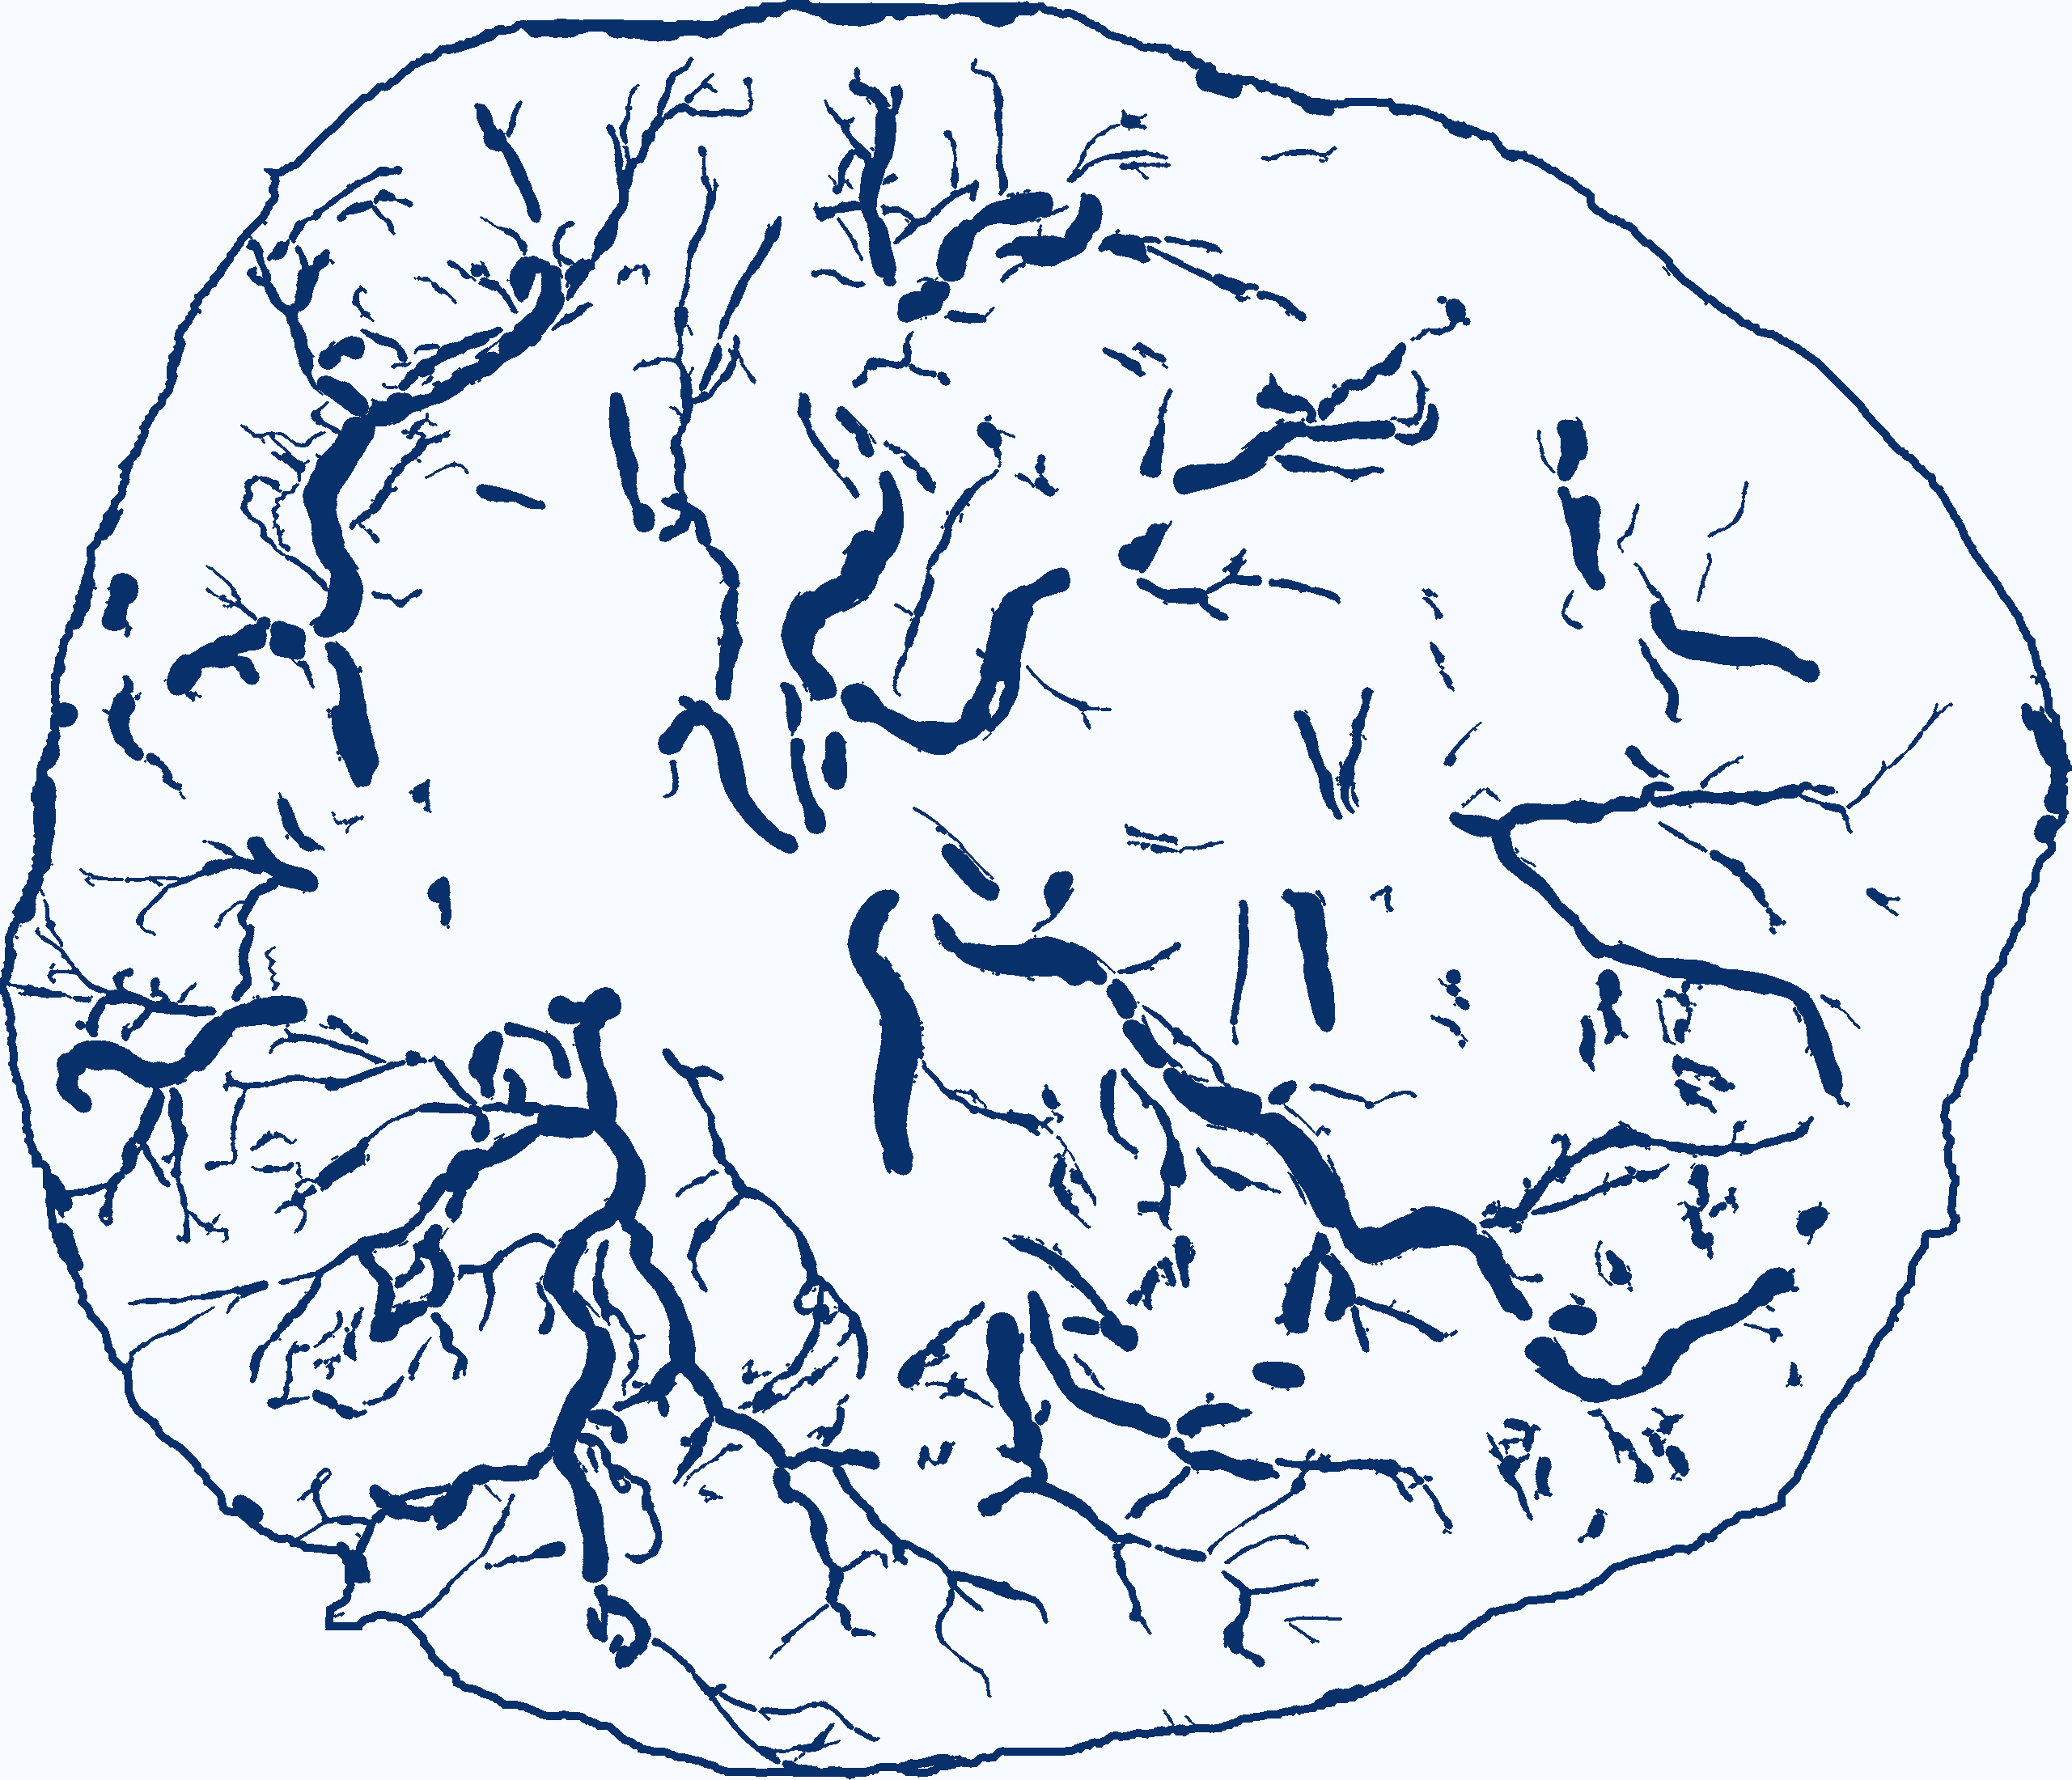
\includegraphics[width=\textwidth]{G-on_skel}
			\caption{Sieving (a) through (b)}
		\end{subfigure}
		\caption{Morphological Filtering (smaller scales only)}
	\end{figure}
\end{frame}


\end{document}

